%%%%%%%%%%%%%%%%%%%%%%%%%%%%%%%%%%%%%%%%%
% Beamer Presentation
% LaTeX Template
% Version 1.0 (10/11/12)
%
% This template has been downloaded from:
% http://www.LaTeXTemplates.com
%
% License:
% CC BY-NC-SA 3.0 (http://creativecommons.org/licenses/by-nc-sa/3.0/)
%
%%%%%%%%%%%%%%%%%%%%%%%%%%%%%%%%%%%%%%%%%

%----------------------------------------------------------------------------------------
%	PACKAGES AND THEMES
%----------------------------------------------------------------------------------------

\documentclass{beamer}

%% \mode<presentation> {

% The Beamer class comes with a number of default slide themes
% which change the colors and layouts of slides. Below this is a list
% of all the themes, uncomment each in turn to see what they look like.

%\usetheme{default}
%\usetheme{AnnArbor}
%\usetheme{Antibes}
%\usetheme{Bergen}
%\usetheme{Berkeley}
%\usetheme{Berlin}
%\usetheme{Boadilla}
%\usetheme{CambridgeUS}
%\usetheme{Copenhagen}
%\usetheme{Darmstadt}
%\usetheme{Dresden}
%\usetheme{Frankfurt}
%\usetheme{Goettingen}
%\usetheme{Hannover}
%\usetheme{Ilmenau}
%\usetheme{JuanLesPins}
%\usetheme{Luebeck}
\usetheme{Madrid}
%% \usetheme{Malmoe}
%\usetheme{Marburg}
%\usetheme{Montpellier}
%% \usetheme{PaloAlto}
%\usetheme{Pittsburgh}
%\usetheme{Rochester}
%\usetheme{Singapore}
%\usetheme{Szeged}
%% \usetheme{Warsaw}

% As well as themes, the Beamer class has a number of color themes
% for any slide theme. Uncomment each of these in turn to see how it
% changes the colors of your current slide theme.

%\usecolortheme{albatross}
%\usecolortheme{beaver}
%\usecolortheme{beetle}
%\usecolortheme{crane}
%\usecolortheme{dolphin}
%\usecolortheme{dove}
%\usecolortheme{fly}
%\usecolortheme{lily}
%\usecolortheme{orchid}
%\usecolortheme{rose}
%\usecolortheme{seagull}
%\usecolortheme{seahorse}
%\usecolortheme{whale}
%\usecolortheme{wolverine}

%\setbeamertemplate{footline} % To remove the footer line in all slides uncomment this line
%% \setbeamertemplate{footline}[page number] % To replace the footer line in all slides with a simple slide count uncomment this line

\setbeamertemplate{navigation symbols}{} % To remove the navigation symbols from the bottom of all slides uncomment this line
%% }

% Captions
\setbeamertemplate{caption}[numbered]
\setbeamerfont{caption}{size=\footnotesize}

% Language and fonts
\usepackage[T2A]{fontenc}
\usepackage[utf8]{inputenc}
\usepackage[english,russian]{babel}

\usepackage{fontspec}
\setmainfont[Ligatures={TeX,Historic}]{Liberation Serif}
\setsansfont{Liberation Sans}
\setmonofont{Liberation Mono}
\usefonttheme{professionalfonts}
\usefonttheme{serif}

% References
\usepackage[
    backend=biber,
    bibencoding=utf8,
    sorting=none,
    sortcites=true,
    bibstyle=gost-numeric,
    citestyle=authortitle-ticomp,
    autolang=other
]{biblatex}

\usepackage{graphicx} % Allows including images
\usepackage{booktabs} % Allows the use of \toprule, \midrule and \bottomrule in tables
\usepackage{appendixnumberbeamer}

\DeclareMathOperator{\argmin}{argmin}
\DeclareMathOperator{\argmax}{argmax}

% Footcites in columns
\addtobeamertemplate{footnote}{\vspace{-6pt}\advance\hsize-0.5cm}{\vspace{6pt}}
\makeatletter
% Alternative A: footnote rule
\renewcommand*{\footnoterule}{\kern -3pt \hrule \@width 2in \kern 8.6pt}
% Alternative B: no footnote rule
% \renewcommand*{\footnoterule}{\kern 6pt}
\makeatother

\addbibresource{master-thesis.bib}

%----------------------------------------------------------------------------------------
%	TITLE PAGE
%----------------------------------------------------------------------------------------

% The short title appears at the bottom of every slide, the full title is only on the title page
\title[DQN-LE-routing]{
  Децентрализованный алгоритм управления конвейерной системой
  с использованием методов мультиагентного обучения с подкреплением
}

\author[Дмитрий Мухутдинов, М4239]{
  Мухутдинов Дмитрий, группа M4239 \\
  Научный руководитель: Фильченков А. А., к.ф-м.н., доцент ФИТиП \\
  Консультант: Вяткин В.В., д.т.н., профессор ФИТиП
}% Your name
\institute[ИТМО] % Your institution as it will appear on the bottom of every slide, may be shorthand to save space
{
  Факультет Информационных Технологий и Программирования \\
  Мегафакультет Трансляционных Информационных Технологий \\
  Университет ИТМО, Санкт-Петербург
}
\date{\today} % Date, can be changed to a custom date

\graphicspath{{img/}{live_img/}}

\begin{document}

\frame{\titlepage}

%----------------------------------------------------------------------------------------
%	PRESENTATION SLIDES
%----------------------------------------------------------------------------------------

\begin{frame}
  \frametitle{Конвейерные системы}
  Применения:
  \begin{itemize}
  \item Промышленность
  \item Сортировка грузов
  \item Распределение багажа
  \item ...
  \end{itemize}
  Типы:
  \begin{itemize}
  \item Для насыпных грузов
  \item Для штучных грузов
    \begin{itemize}
    \item В т. ч. для транспортировки багажа
    \end{itemize}
  \end{itemize}
\end{frame}

%------------------------------------------------

\begin{frame}
  \frametitle{Задача управления конвейерной системой}
  Подзадачи:
  \begin{itemize}
  \item Собственно доставка грузов
    \begin{itemize}
    \item Является задачей маршрутизации
    \end{itemize} 
  \item Избежание столкновения грузов
  \item Оптимизация энергопотребления
  \end{itemize}
\end{frame}

\begin{frame}
  \frametitle{Управления конвейерной системой: маршрутизация}
  \begin{itemize}
  \item Для насыпных грузов: оптимальный контроль по заданному расписанию\footcite{ago2007simultaneous}
    \begin{itemize}
    \item Множество запросов маршрутизации $\{(s_i, d_i)\}_{t=0}^T$ за промежуток времени $T$ --- параметр глобальной оптимизационной задачи
    \item Обычно сводится к задаче линейного/квадратичного программирования.
    \end{itemize} 
  \item Для штучных грузов (багажные системы):
    \begin{itemize}
    \item Оптимальный контроль нецелесообразен
      \begin{itemize}
      \item Пассажиры сдают багаж в случайном порядке
      \end{itemize} 
    \item Централизованный статический роутинг (BSR\footcite{johnstone2009status})
    \item Децентрализованный роутинг на основе distance-vector протокола\footcite{black2009intelligent}
    \end{itemize} 
  \item Закрытые проприетарные подходы от компаний-производителей (в обоих случаях)
  \end{itemize}
\end{frame}

\begin{frame}
  \frametitle{Управления конвейерной системой: избежание столкновений}
  \begin{itemize}
  \item При оптимальном контроле (в насыпных конвейерах): вводится как одно из ограничений оптимизационной задачи\footcite{ago2007simultaneous}
  \item Для штучных грузов:
    \begin{itemize}
    \item Одна идея: взаимная синхронизация скоростей сочленяющихся конвейеров
    \item Кто-то это патентует\footcite{schafer2011material}
    \item Описан в рамках децентрализованного контроля у Вяткина\footcite{black2009intelligent}
    \end{itemize}
  \end{itemize}
\end{frame}

\begin{frame}
  \frametitle{Управления конвейерной системой: энергосбережение}
  \begin{itemize}
  \item Для насыпных грузов:
    \begin{itemize}
    \item Стандартные модели энергопотребления: ISO 5048, DIN 22101, JIS B 9905 (сложные)
    \item Упрощенные модели для оптимизации на их основе\footcite{zhang2011modeling}
    \item Оптимальный контроль по заданному расписанию:
      \begin{itemize}
      \item Включение-выключение питания\footcite{middelberg2009optimal}
      \item Управление скоростью\footcite{zhang2010optimal} (эффективнее)
      \end{itemize}
    \end{itemize}
  \item Для штучных грузов:
    \begin{itemize}
    \item Простая абстрактная модель энергопотребления\footcite{halepoto2016design}
      \begin{itemize}
      \item Постулируется линейная зависимость от скорости конвейера и \textit{некоторая} -- от массы грузов на нем
      \end{itemize} 
    \end{itemize} 
  \end{itemize}
\end{frame}

\begin{frame}
  \frametitle{Децентрализованный подход (Вяткин)}
  \begin{columns}
    \begin{column}{0.5\textwidth}
      \begin{itemize}
      \item В рамках стандарта IEC 61499
      \item Контроллер одного конвейера -- независимый агент
        \begin{itemize}
        \item Оснащен датчиком скорости, детекторами сумок у развилок и отклонителями на исходящих развилках
        \item Управляет скоростью и отклонителями
        \item Моделирует позиции собственных сумок
        \end{itemize}
      \item Маршрутизация на основе distance-vector
      \item Протокол для избежания столкновений
      \end{itemize}
    \end{column}
    \begin{column}{0.5\textwidth}
      \begin{center}
        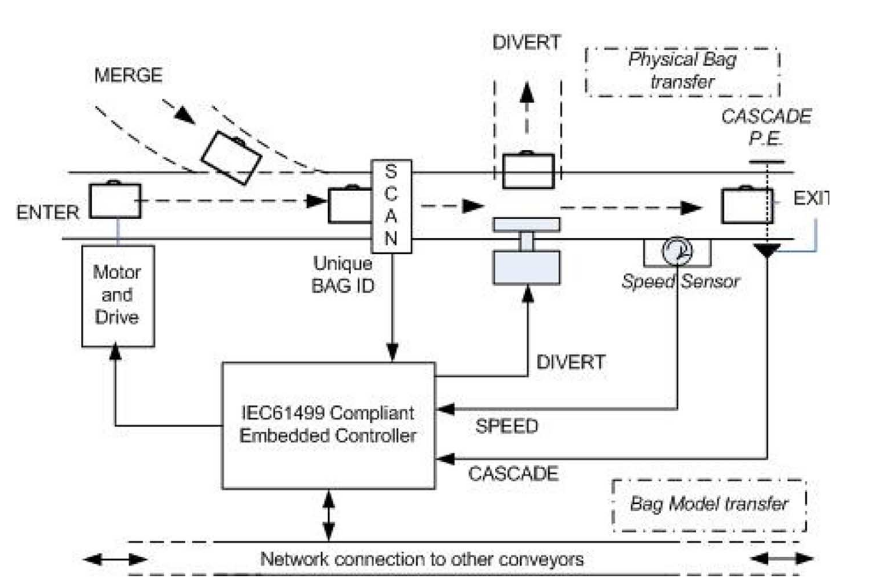
\includegraphics[width=\textwidth]{vyatkin-conveyors-illustration}
        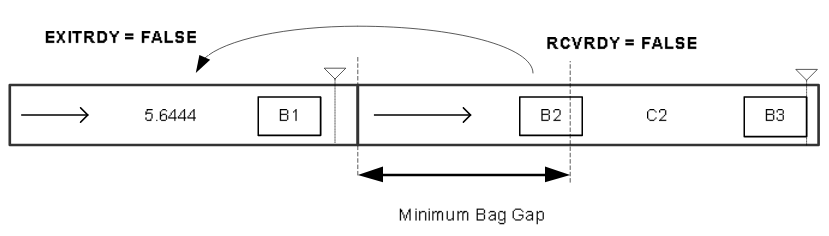
\includegraphics[width=\textwidth]{collision-avoidance-1}
      \end{center}
    \end{column}
  \end{columns}
\end{frame}

%------------------------------------------------

\begin{frame}
  \frametitle{Цель работы}
  Разработать метод управления конвейерной системой со следующими свойствами:
  \begin{itemize}
  \item Децентрализованность
  \item Решение всех перечисленных подзадач: маршрутизации, избежания столкновений и энергоcбережения
  \item Устойчивость к разнородным изменениям в условиях среды
    \begin{itemize}
    \item Изменения характеристик багажного потока
    \item Поломки конвейеров
    \end{itemize}
  \end{itemize}
\end{frame}

%-------------------------------------------------

\begin{frame}
  \frametitle{Идея}
  \begin{itemize}
  \item Предполагаем оборудование аналогичное описанному у Вяткина
    \begin{itemize}
    \item Один конвейер -- один контроллер
    \item Единственное дополнительное предположение: счетчик электроэнергии
    \end{itemize}
  \item Аналогичный протокол для избежания столкновений
  \item Постановка задачи в терминах RL
  \item Нейросети в качестве маршрутизаторов для каждого сочленения
     \begin{itemize}
     \item Логика маршрутизатора - универсальная, может использоваться и в компьютерных сетях
     \end{itemize}
  \item Маршрутизация на основе Q-routing\footcite{q-routing-orig}
  \end{itemize}
\end{frame}

%------------------------------------------------

\begin{frame}
  \frametitle{Постановка задачи в терминах RL}
  \begin{itemize}
    \item Формально, агентом в сети является \textit{сумка}
    \item Действие --- перенаправление в развилке отклонителем
    \item Выключаем конвейеры без сумок
      \begin{itemize}
      \item $r_t = (t_d - t_s) + \alpha\int_{t_l^k}^{t_d} \! p_k(t) \; \mathrm{d}t$
      \item Оверхэд рассчитывается принимающим конвейером
      \end{itemize}

    \item Вознаграждение сумки состоит из времени перемещения и оверхэда на энергопотребление:
      \begin{itemize}
      \item $r_t = (t_d - t_s) + \alpha\int_{t_s}^{t_d} \! p_k(t) \; \mathrm{d}t$
      \item Оверхэд рассчитывается принимающим конвейером
      \end{itemize}
  \end{itemize}
\end{frame}

%----------------------------------------------------------------

\begin{frame}
  \frametitle{Что было сделано: алгоритм DQN-routing\footcite{mukhutdinov2019multi}}
  \begin{columns}
    \begin{column}{0.6\textwidth}
      \begin{itemize}
      \item Объединяет link-state протокол с алгоритмом Q-routing
      \item Вход нейросети:
        \begin{itemize}
        \item Текущий узел $n$, узел назначения $d$
        \item Узлы-соседи $Y$
        \item Матрица смежности графа
        \end{itemize}
      \item Выход: $\{ Q_x(d, y) \}_{y \in Y}$
      \end{itemize}
      Был протестирован в сеттинге компьютерных и конвейерных сетей
    \end{column}
    \begin{column}{0.4\textwidth}
      \begin{center}
        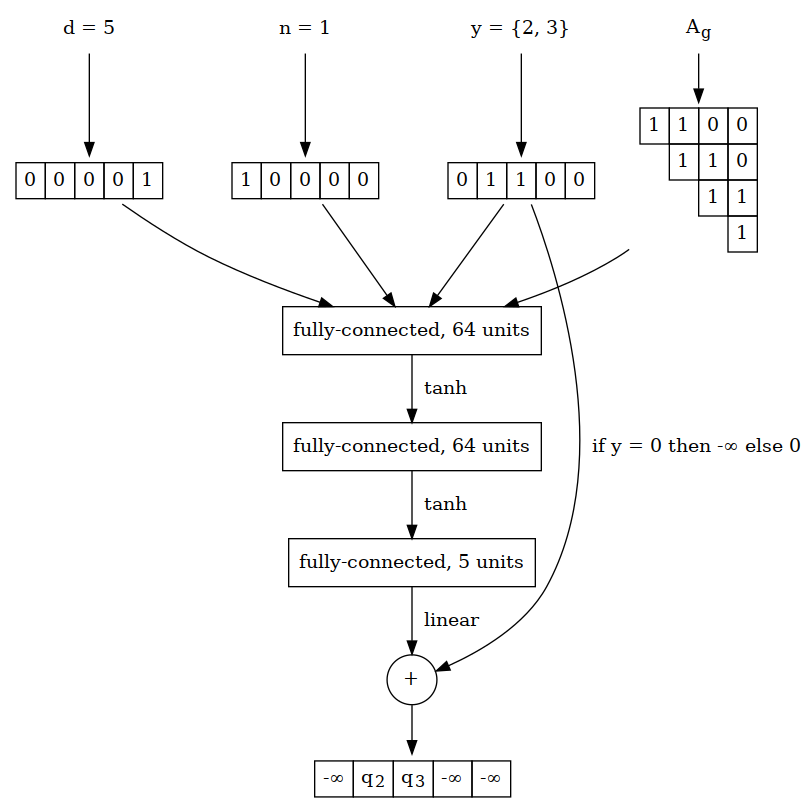
\includegraphics[width=\textwidth]{nn-2}
      \end{center}
    \end{column}
  \end{columns}
\end{frame}

%----------------------------------------------------------------

\begin{frame}
  \frametitle{Плюсы и минусы DQN-routing}
  \begin{itemize}
  \item Плюсы
    \begin{itemize}
    \item Адаптация под изменения трафика
    \item Адаптация после поломок
    \item Оптимизация времени доставки и энергопотребления с заданным приоритетом
    \end{itemize}
  \item Минусы
    \begin{itemize}
    \item Размер выходного слоя линейно зависит от размера графа
    \item Размер входного слоя квадратично (!) зависит от размера графа
    \item Требует предварительного обучения с учителем
    \end{itemize}
  \end{itemize}
  Можно ли избавиться от минусов, не потеряв плюсов?
\end{frame}

%----------------------------------------------------------------

\begin{frame}
  \frametitle{Идеи усовершенствования алгоритма}
  \begin{itemize}
  \item Предсказание Q-функции отдельно для каждого исходящего ребра
    \begin{itemize}
    \item Вместо множества текущих соседей подаем на вход одного соседа $y$.
    \item Один нейрон на выходном слое выдает скалярное значение $Q_x(d, y)$
    \end{itemize}

  \item Использование графовых эмбеддингов
    \begin{itemize}
    \item Вместо кодирования меток узлов унитарным кодом использовать их
      отображения в векторное пространство фиксированной размерности
    \item Отказ от подачи на вход матрицы смежности
      \begin{itemize}
      \item Вместо этого пересчитывать эмбеддинги при изменении топологии
      \item Эмбеддинги косвенно передадут информацию о топологии
      \end{itemize}
    \end{itemize}
  \end{itemize}
\end{frame}

%----------------------------------------------------------------

\begin{frame}
  \frametitle{Модификация: DQN-LE-routing}
  \begin{columns}
    \begin{column}{0.6\textwidth}
      \begin{itemize}
      \item Получаем эмбеддинги методом Laplacian Eigenmaps (LE)
      \item Нормализуем веса ребер по среднему перед расчетом
      \item Полученные эмбеддинги домножаем на средний вес
      \end{itemize}

      Тогда
      \begin{align*}
        Q_n(d, y) = f_{\theta}( &(LE_G(d) - LE_G(n)) \odot \\
                             &(LE_G(y) - LE_G(n)))
      \end{align*}

      , где:
      \begin{itemize}
      \item $LE_G(\cdot)$ возвращает эмбеддинг по номеру узла
      \item $f_{\theta}(\cdot)$ --- feed-forward нейронная сеть
      \end{itemize}
    \end{column}
    \begin{column}{0.4\textwidth}
      \begin{center}
        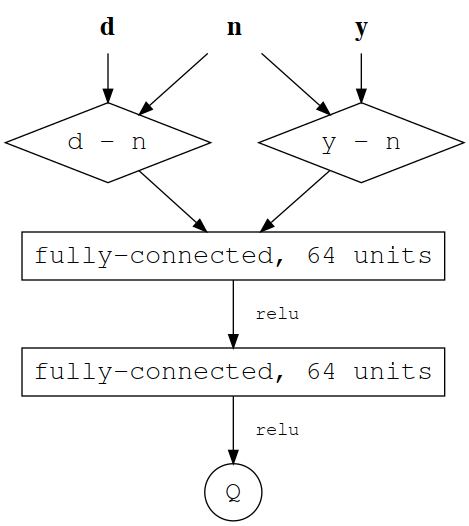
\includegraphics[width=\textwidth]{nn-1-one-out.png}
      \end{center}
    \end{column}
  \end{columns}
\end{frame}

%----------------------------------------------------------------

\begin{frame}
  \frametitle{Эксперименты в модели компьютерной сети}
  \begin{itemize}
  \item Запуск экспериментов в симуляторе
  \item Размерность эмбеддинга: 8
  \item Бейзлайны:
    \begin{itemize}
    \item Табличный Q-routing
    \item Дейкстра с протоколом link-state (shortest paths, SP)
    \item Оригинальный DQN-routing (DQN)
    \end{itemize}
  \item Служебные сообщения доставляются бесплатно
  \item Зачем?
    \begin{itemize}
    \item Быстрее симулировать, чем конвейеры
    \item Показываем универсальность алгоритма
    \end{itemize}
  \end{itemize}
\end{frame}

\begin{frame}
  \frametitle{Эксперименты в модели компьютерной сети: предобучение}
  \begin{columns}
    \begin{column}{0.5\textwidth}
      \begin{itemize}
      \item У нетабличного Q-обучения нет гарантий сходимости (\ref{fig:dqn-no-pretrain})
      \item Experience replay не работает в нестационарной среде
      \item Предобучаем на действиях алгоритма shortest paths
      \item Получаем данные на базовом графе (\ref{fig:network-small}) и его модификациях
      \end{itemize}
    \end{column}
    \begin{column}{0.5\textwidth}
      \begin{center}
        \begin{figure}[!h]
          \caption{Базовая топология сети для тестов}\label{fig:network-small}
          \centerline{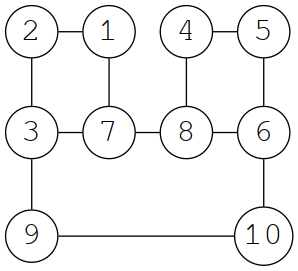
\includegraphics[width=0.4\textwidth]{graph-2-1.png}}
        \end{figure}        
        \vspace{-0.4in}
        \begin{figure}[!h]
          \caption{Работа DQN без предобучения}\label{fig:dqn-no-pretrain}
          \centerline{\includegraphics[width=\textwidth]{dqn-no-pretrain-small}}
        \end{figure}
      \end{center}
    \end{column}
  \end{columns}
\end{frame}


%------------------------------------------------------

\begin{frame}
  \frametitle{Эксперименты: резкое изменение нагрузки}
  \includegraphics[width=\textwidth]{peak-load-small} 
\end{frame}

%------------------------------------------------------

\begin{frame}
  \frametitle{Эксперименты: обрыв и восстановление соединений}
  \includegraphics[width=\textwidth]{topology-change-small} 
\end{frame}

%------------------------------------------------------

\begin{frame}
  \frametitle{Перенос опыта на новую топологию}
  \begin{columns}
    \begin{column}{0.5\textwidth}
      \begin{itemize}
      \item DQN-LE-routing все еще требует предобучения
      \item Однако, если опыт переносится на совершенно новые топологии, это не страшно
      \item Проверим производительность на случайном графе 
      \end{itemize}
    \end{column}
    \begin{column}{0.5\textwidth}
      \begin{center}
          \centerline{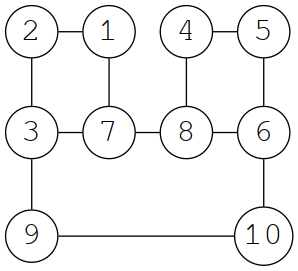
\includegraphics[width=0.4\textwidth]{graph-2-1.png}}
          \centerline{\Big\downarrow}
          \centerline{\includegraphics[width=\textwidth]{random-graph-10n}}
      \end{center}
    \end{column}
  \end{columns}
\end{frame}

%------------------------------------------------------

\begin{frame}
  \frametitle{Перенос опыта на новую топологию: то же кол-во вершин}
  \includegraphics[width=\textwidth]{learning-transfer-small} 
\end{frame}

%------------------------------------------------------

\begin{frame}
  \frametitle{Перенос опыта на новую топологию: большее кол-во вершин}
  \begin{columns}
    \begin{column}{0.3\textwidth}
      \centerline{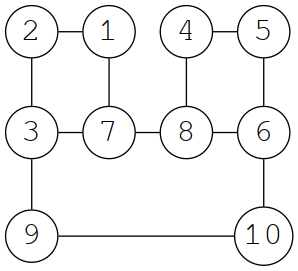
\includegraphics[width=0.8\textwidth]{graph-2-1.png}}
    \end{column}
    \begin{column}{0.1\textwidth}
      $\hbox{\fontsize{1in}{1in}\selectfont\(\Rightarrow\)}$
    \end{column}
    \begin{column}{0.6\textwidth}
      \centerline{\includegraphics[width=\textwidth]{random-graph-40n}}
    \end{column}
  \end{columns}
\end{frame}

%------------------------------------------------------

\begin{frame}
  \frametitle{Перенос опыта на новую топологию: большее кол-во вершин}
  \begin{columns}
    \begin{column}{0.5\textwidth}
      \begin{figure}[!h]
        \centerline{\includegraphics[width=\textwidth]{learning-transfer-big-low-load}}
        \caption{Низкая нагрузка}
      \end{figure}
    \end{column}
    \begin{column}{0.5\textwidth}
      \begin{figure}
        \centerline{\includegraphics[width=\textwidth]{learning-transfer-big-high-load}}
        \caption{Высокая нагрузка}
      \end{figure}
    \end{column}
  \end{columns}
\end{frame}

%------------------------------------------------------

\begin{frame}
  \frametitle{Эксперименты в модели конвейерной системы}
  \begin{itemize}
  \item Бейзлайны:
    \begin{itemize}
    \item Оригинальный децентрализованный подход Вяткина (обозн. Vyatin-Black)
    \item Централизованный статический роутинг (BSR\footcite{johnstone2009status})
      \begin{itemize} 
      \item Плюс централизованное избежание столкновений по аналогии с Vyatkin-Black (самописное, нет в оригинале)
      \end{itemize}
    \item Модификация Vyatkin-Black с использованием табличного Q-routing
    \end{itemize}
  \item Заданы параметры:
    \begin{itemize}
    \item Длины и максимальные скорости конвейеров
    \item Задержка перед остановкой после ухода сумок с конвейера
    \item Конфигурация системы: входы, выходы и сочленения
    \end{itemize}
  \item Модель энергопотребления: модель от Zhang для насыпных конвейеров, адаптированная для штучных
    \begin{itemize}
    \item $P(V, T) = \frac{1}{\eta} \left( \theta_1 VT^2 + \theta_2 V + \theta_3 \frac{T^2}{V} + \theta_4 T + \frac{V^2T}{3.6} \right)$
    \item $T = M_b * V * 3.6 / L$ 
    \item $V$ -- скорость, $M_b$ -- масса всех сумок, $L$ -- длина конвейера
    \end{itemize} 
  \end{itemize}
\end{frame}

%------------------------------------------------------

\begin{frame}
  \frametitle{Модель конвейерной системы для проведения экспериментов}
  \begin{center}
    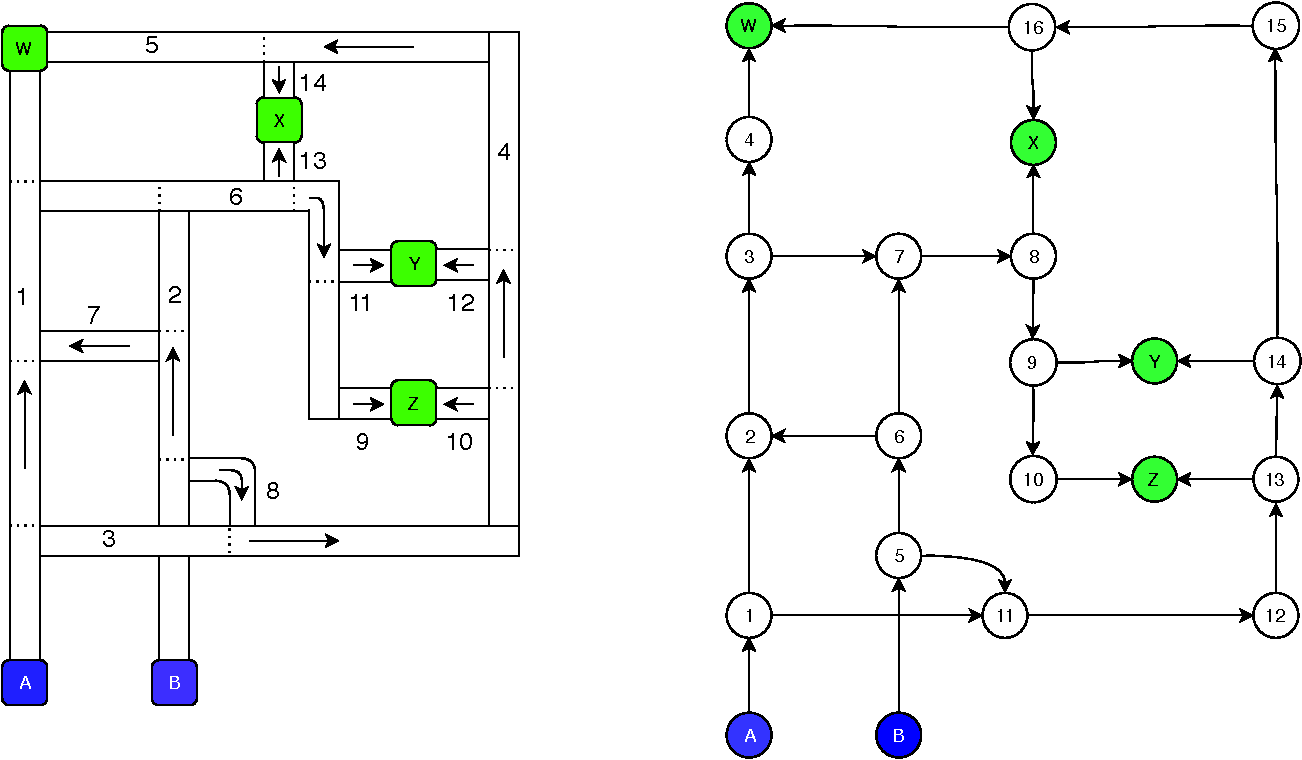
\includegraphics[width=0.9\textwidth]{conveyor-1-illustration-2} 
  \end{center}
\end{frame}

%------------------------------------------------------

\begin{frame}
  \frametitle{Неравномерный поток до выходных вершин}
  \begin{columns}
    \begin{column}{0.5\textwidth}
      \includegraphics[width=\textwidth]{conveyors-new-1-time}
    \end{column}
    \begin{column}{0.5\textwidth}
      \includegraphics[width=\textwidth]{conveyors-new-1-energy}
    \end{column}
  \end{columns}
\end{frame}

%------------------------------------------------------

%-------------------------------------------------------

\begin{frame}
  \frametitle{Итоги}
  \begin{itemize}
  \item Разработана модификация алгоритма DQN-routing --- DQN-LE-routing
  \item Модифицированный алгоритм свободен от ключевых недостатков DQN-routing:
    \begin{itemize}
    \item Зависимость размера нейронной сети от размера графа
    \item Необходимость переобучения с учителем на новых графах
    \end{itemize}
  \item Превосходит изначальный алгоритм по качеству работы и границам применимости
    \begin{itemize}
    \item Также работает быстрее ввиду меньшего размера нейросети
    \item Гораздо лучше подходит для микроконтроллерной реализации
    \end{itemize}
  \end{itemize}
\end{frame}

%-------------------------------------------------------
%-------------------------------------------------------

%% \begin{frame}
%%   \frametitle{Иcпользование графовых эмбеддингов: результаты}
%%   Алгоритм HOPE\footcite{ou2016asymmetric} с использованием Katz index как
%%   метрики похожести.
%%   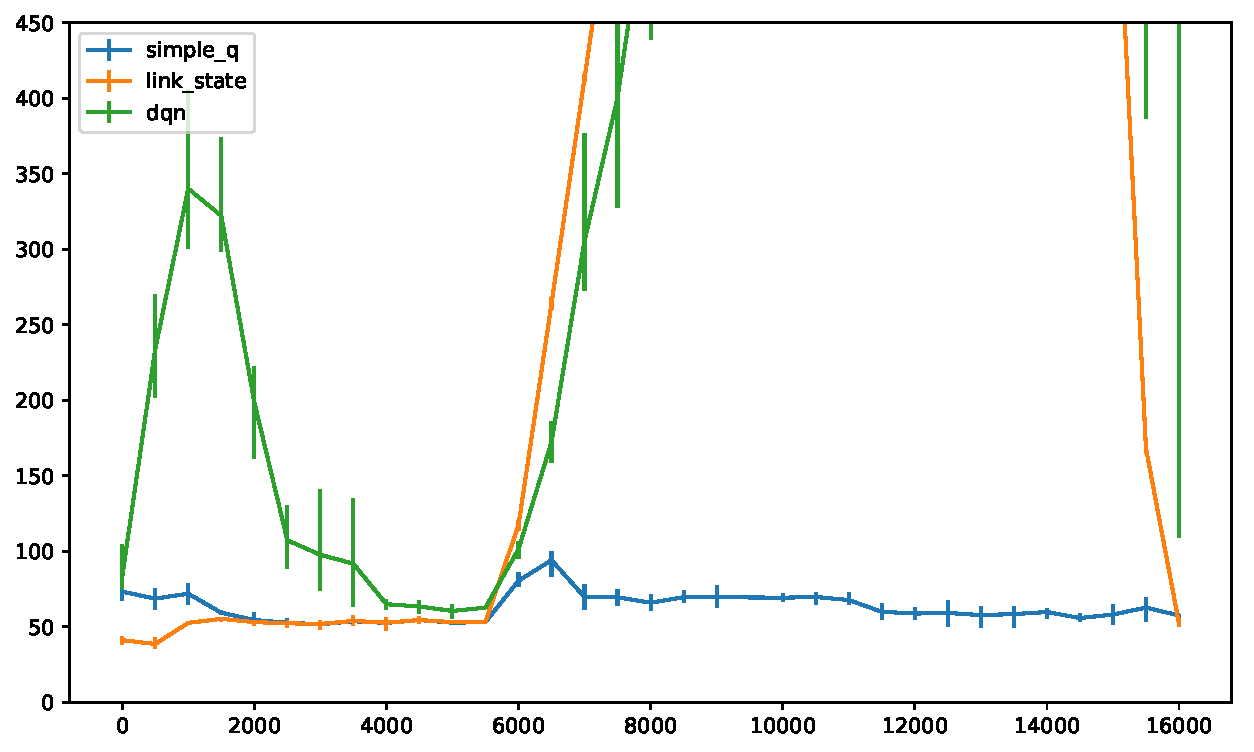
\includegraphics[width=0.8\textwidth]{peak-load-embedding} \\
%%   :(
%% \end{frame}

%-------------------------------------------------------

%% \begin{frame}
%%   \frametitle{Зональная маршрутизация: идея}
%%   \begin{columns}
%%     \begin{column}{0.6\textwidth}
%%       \begin{itemize}
%%       \item Ограничиваем рассматриваемый граф только узлами не далее $k$ ребер от
%%         данного 
%%       \item Если узел назначения находится вне текущей зоны --- делаем запрос к
%%         узлам на границе зоны.
%%       \end{itemize}
%%     \end{column}
%%     \begin{column}{0.4\textwidth}
%%       \begin{center}
%%         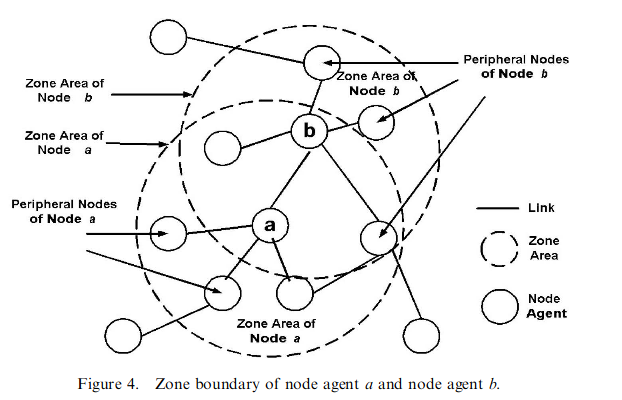
\includegraphics[width=\textwidth]{zone-routing}
%%       \end{center}
%%     \end{column}
%%   \end{columns}
%% \end{frame}

%% \begin{frame}
%%   \frametitle{Зональная маршрутизация: результаты}
%%   \huge{:shrug:}
%% \end{frame}

%-------------------------------------------------------

%% \begin{frame}
%%   \frametitle{Глобальная графовая нейронная сеть: результаты}
%%   \huge{:shrug:}
%% \end{frame}

%-------------------------------------------------------

%% \begin{frame}
%%   \frametitle{Итоги}
%%   \begin{itemize}
%%   \item :shrug:
%%   \end{itemize}
%% \end{frame}

%-------------------------------------------------------

%% \begin{frame}
%%   \frametitle{Направления дальнейших исследований}
%%   \begin{itemize}
%%   \item Поиск/изобретение более качественных бейзлайнов (например, на основе MPC)
%%   \item Исследование идеи глобальной графовой нейронной сети\footcite{scarselli2009graph}\footcite{li2015gated}\footcite{geyer2018learning}
%%   \item Проведение большего числа экспериментах на различных топологиях
%%     \begin{itemize}
%%       \item В т. ч. случайная генерация правдоподобных конвейерных сетей
%%     \end{itemize}
%%   \item Выход за пределы маршрутизации
%%     \begin{itemize}
%%       \item Обучение контроллера скорости конвейера
%%     \end{itemize} 
%%   \end{itemize}
%% \end{frame}

%-------------------------------------------------------

\begin{frame}
  \begin{center}
    {\Huge Спасибо за внимание!}
  \end{center}
\end{frame}

\appendix
\begin{frame}
  \frametitle{Плавное повышение нагрузки: $\alpha = 5e6$}
  \begin{columns}
    \begin{column}{0.5\textwidth}
      \includegraphics[width=\textwidth]{conveyors-new-2-time}
    \end{column}
    \begin{column}{0.5\textwidth}
      \includegraphics[width=\textwidth]{conveyors-new-2-energy}
    \end{column}
  \end{columns}
\end{frame}

%% \begin{frame}
%%   \frametitle{Глобальная графовая нейронная сеть: идея}
%%   \begin{columns}
%%     \begin{column}{0.6\textwidth}
%%       \begin{itemize}
%%       \item Рассматриваем весь граф с состояниями ребер и узлов как вход для
%%         графовой нейронной сети (GG-NN)
%%       \item Считается распределенно на физических узлах системы
%%       \item Промежуточные состояния и их градиенты передаются между узлами по
%%         сети 
%%         \begin{itemize}
%%         \item Применяется для компьютерных сетей с обучением с учителем\footnotemark
%%         \item Добавим обучение с подкреплением во время работы
%%         \end{itemize} 
%%       \end{itemize}
%%     \end{column}
%%     \begin{column}{0.4\textwidth}
%%       \begin{center}
%%         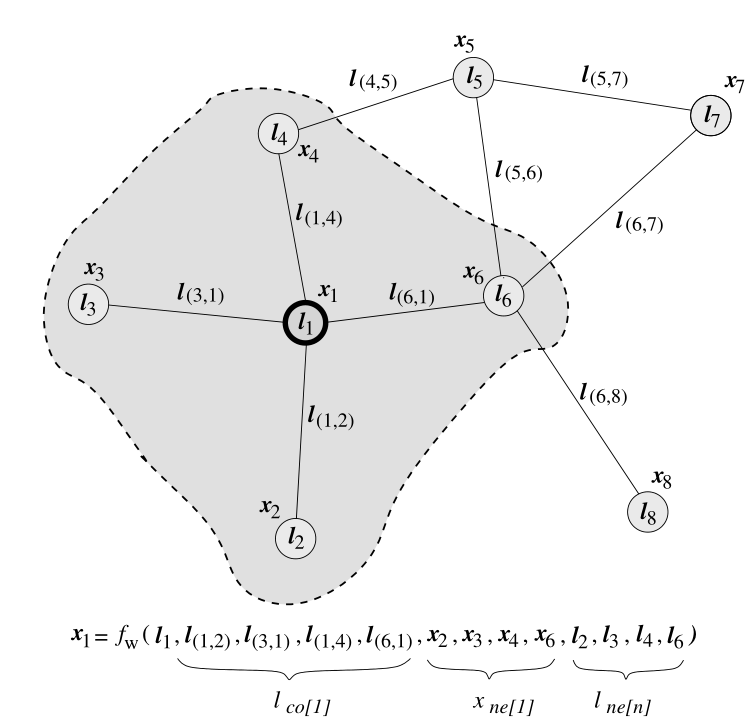
\includegraphics[width=\textwidth]{gnn.png}
%%         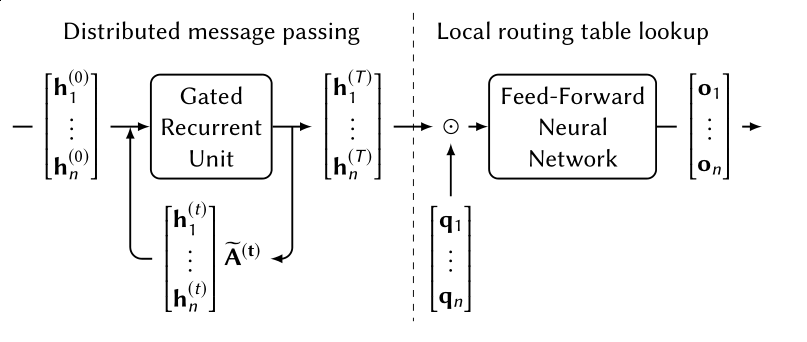
\includegraphics[width=\textwidth]{gg-qnn.png}
%%       \end{center}
%%     \end{column}
%%   \end{columns}
%%   \footcitetext{geyer2018learning}
%% \end{frame}

%% \begin{frame}[allowframebreaks]
%%   \frametitle{Библиография}
%%   \printbibliography
%% \end{frame}

%-------------------------------------------------------

%% \begin{frame}
%%   \frametitle{Иллюстрация несходимости алгоритма к оптимуму без предобучения}
%%   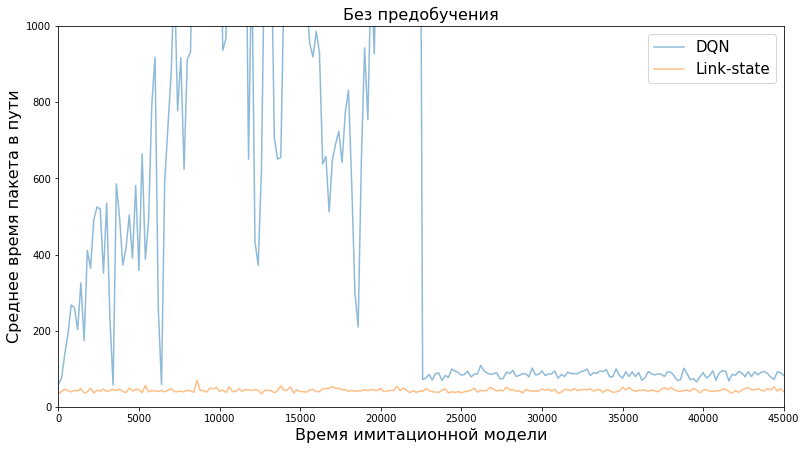
\includegraphics[width=\textwidth]{non-convergence}
%% \end{frame}

%% \begin{frame}
%%   \frametitle{Сравнение алгоритмов оптимизации: скорость предобучения}
%%   \begin{columns}
%%     \begin{column}{0.5\textwidth}
%%       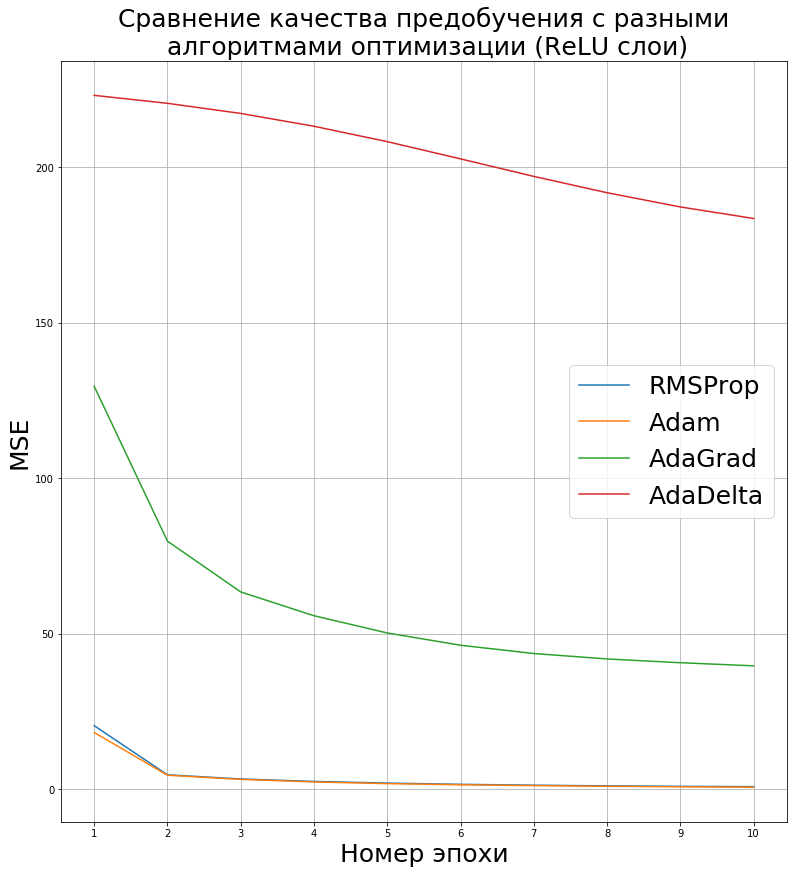
\includegraphics[width=\textwidth]{experiment-optimizers-pretrain-tall}
%%     \end{column}
%%     \begin{column}{0.5\textwidth}
%%       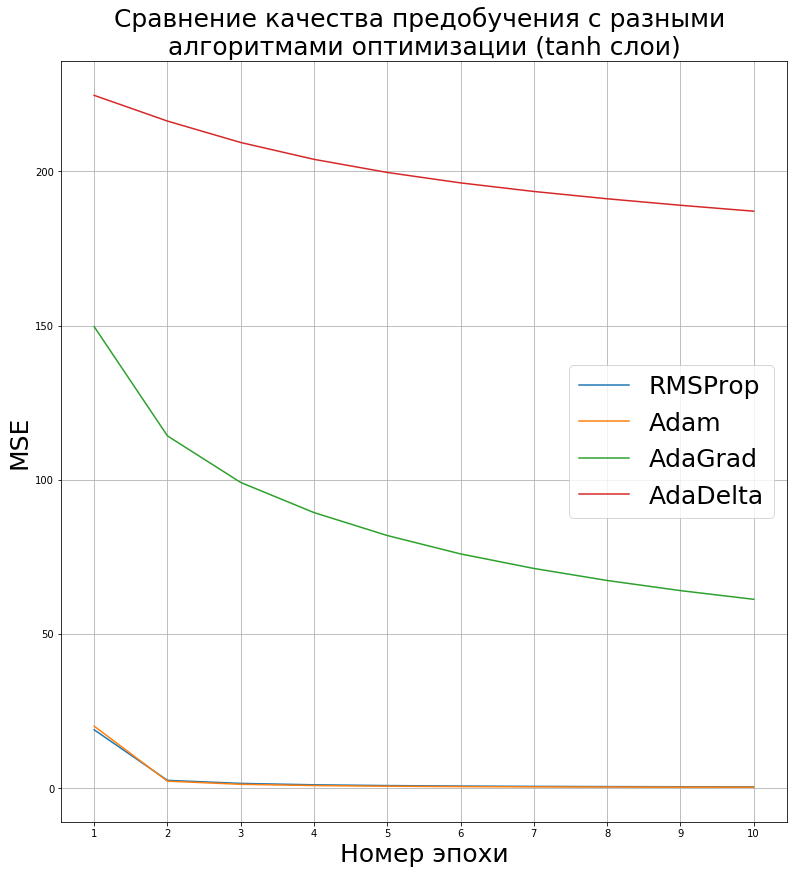
\includegraphics[width=\textwidth]{experiment-optimizers-pretrain-tanh-tall}
%%     \end{column}
%%   \end{columns}
%% \end{frame}

%% \begin{frame}
%%   \frametitle{Сравнение алгоритмов оптимизации и функций активации: скорость предобучения}
%%   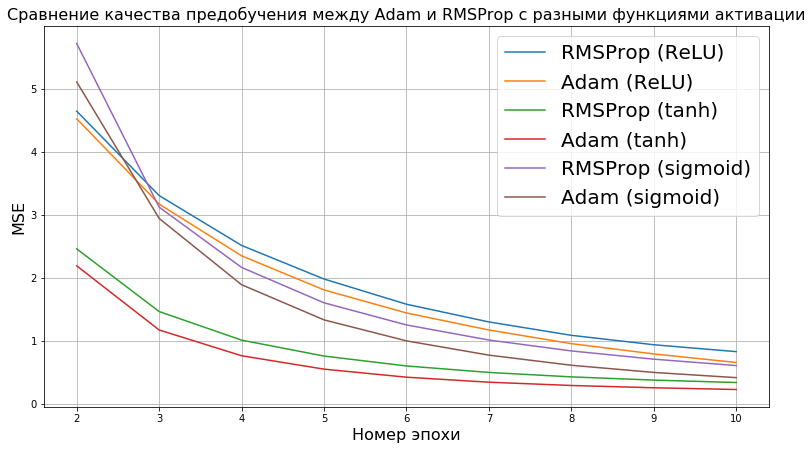
\includegraphics[width=\textwidth]{experiment-optimizers-pretrain-adam-vs-rmsprop}
%% \end{frame}

%% \begin{frame}
%%   \frametitle{Сравнение RMSProp и Adam в модели компьютерной сети}
%%   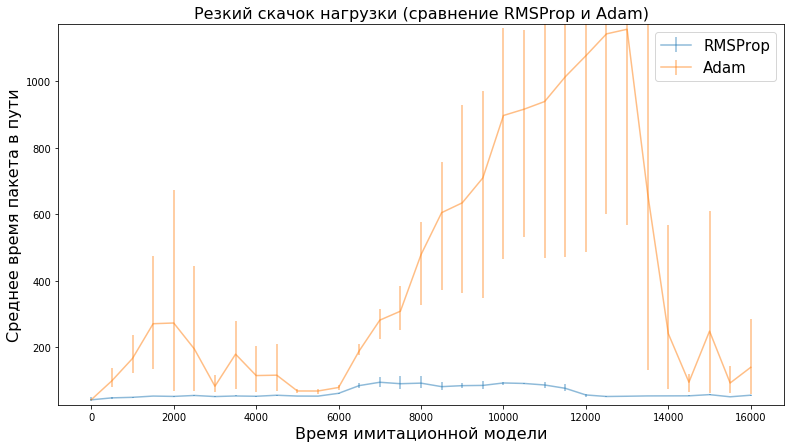
\includegraphics[width=\textwidth]{experiment-adam-failure}
%% \end{frame}

%% \begin{frame}
%%   \frametitle{Сравнение фукнций активации c RMSProp в модели компьютерной сети}
%%   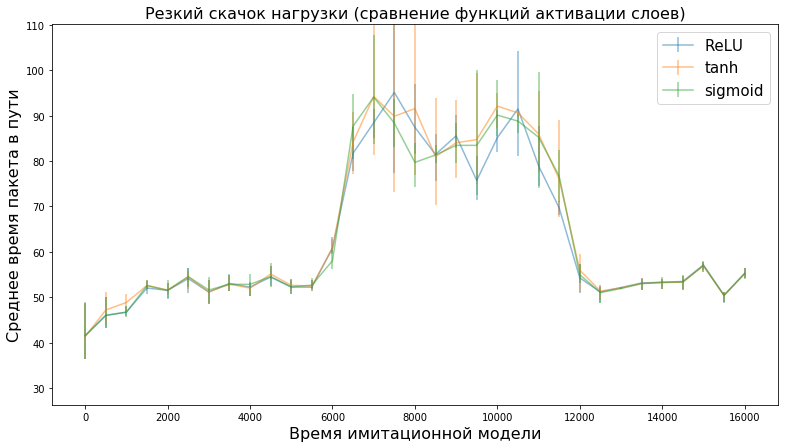
\includegraphics[width=\textwidth]{experiment-activations-launch}
%% \end{frame}

%% \begin{frame}
%%   \frametitle{Сравнение различных конфигураций feed-forward нейросети по
%%     качеству предобучения}
%%   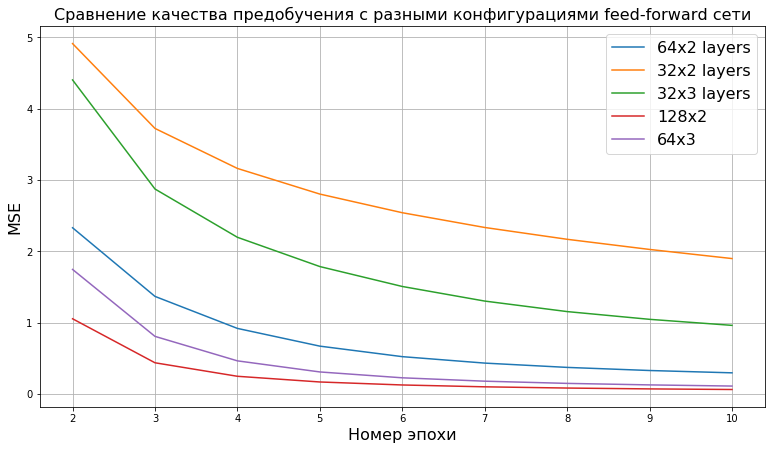
\includegraphics[width=\textwidth]{experiment-layers-pretrain}
%% \end{frame}

%% \begin{frame}
%%   \frametitle{Сравнение различных конфигураций feed-forward нейросети при работе
%%     в имитационной модели}
%%   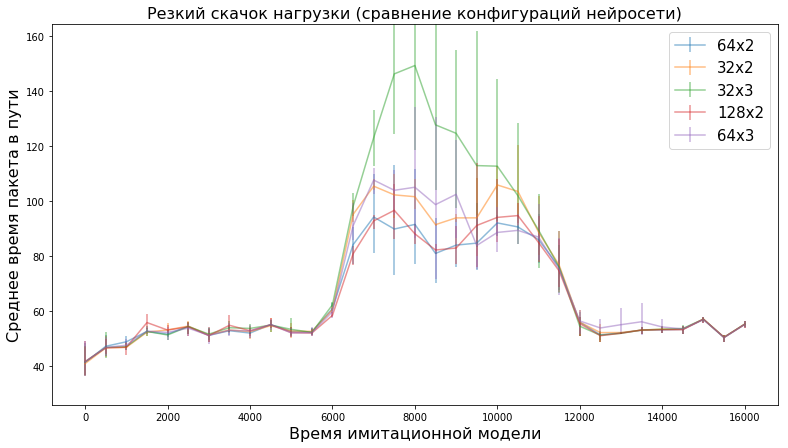
\includegraphics[width=\textwidth]{experiment-layers-launch}
%% \end{frame}

%% \begin{frame}
%%   \frametitle{Влияние softmax-стратегии на работу алгоритма}
%%   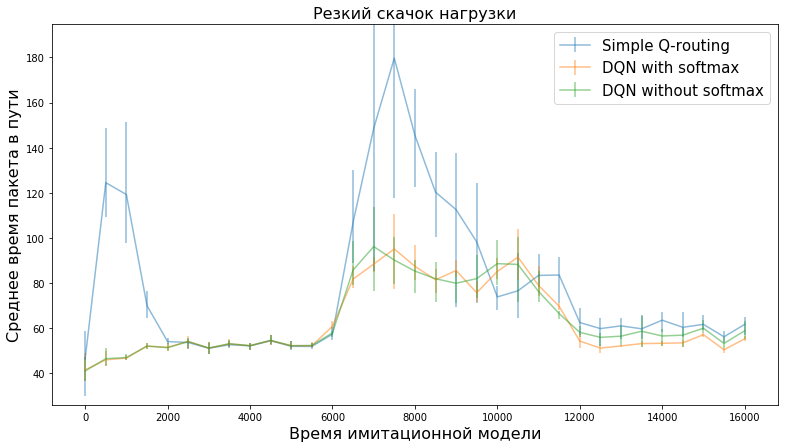
\includegraphics[width=\textwidth]{experiment-softmax-effect}
%% \end{frame}

%% \begin{frame}
%%   \frametitle{Влияние различных видов experience replay на работу алгоритма}
%%   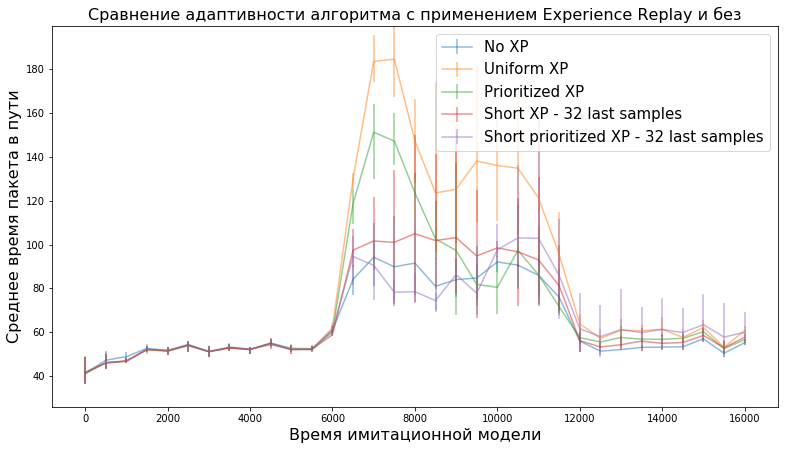
\includegraphics[width=\textwidth]{experiments-xp-variants}
%% \end{frame}

%% \begin{frame}
%%   \frametitle{Влияние включения матрицы смежности в наблюдаемое состояние}
%%   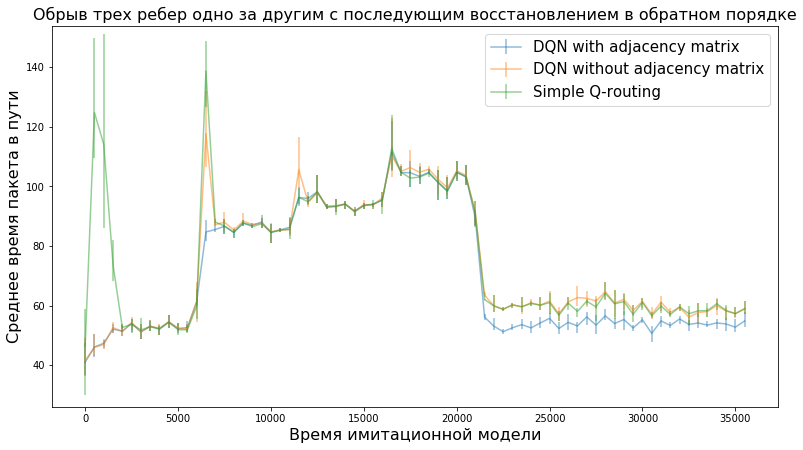
\includegraphics[width=\textwidth]{experiment-with-without-amatrix}
%% \end{frame}

%% \begin{frame}
%%   \frametitle{Влияние включения информации о состоянии соседних конвейеров в
%%     наблюдаемое состояние}
%%   \begin{columns}
%%     \begin{column}{0.5\textwidth}
%%       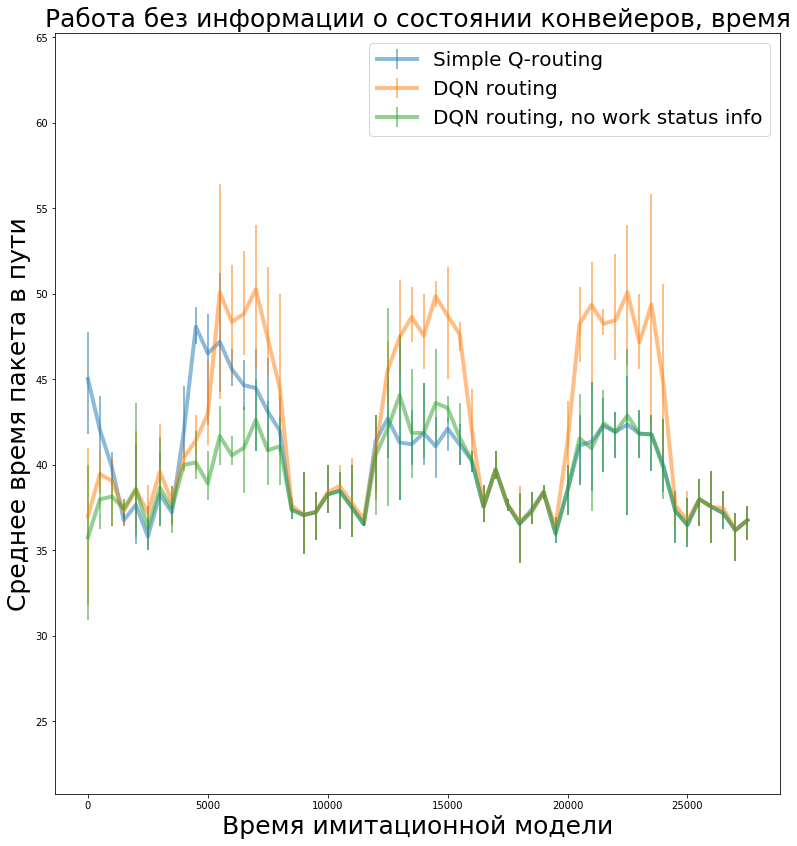
\includegraphics[width=\textwidth]{experiment-conveyors-en1-time-no-ws-tall}
%%     \end{column}
%%     \begin{column}{0.5\textwidth}
%%       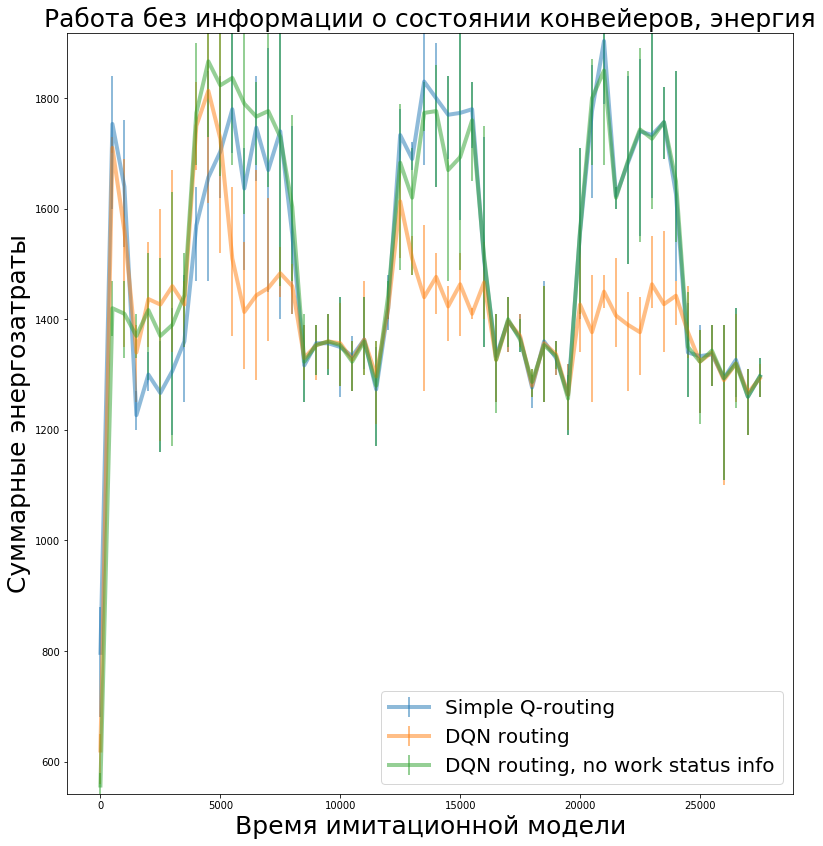
\includegraphics[width=\textwidth]{experiment-conveyors-en1-energy-no-ws-tall}
%%     \end{column}
%%   \end{columns}
%% \end{frame}

\end{document} 
